\chapter{Results of experiments with \sgp}
\label{app:sgp}
\textit{This Appendix, presents graphically a summary of individuals runs using \sgp. Figures show a \textit{box-plot} representation for different strategies and a bar representation for the percentage of winner solvers types.}
\vfill
\newpage

In Figures~\ref{boxplot:5comm}, \ref{boxplot:8comm} and \ref{boxplot:9comm}, labels of the x-axis correspond to the following strategies:
\begin{enumerate}[itemsep=-1mm]
\item \textbf{NC}: Non communication strategy, 
\item \textbf{100SC1-1}: 100\% of communicating solvers performing simple communication \oneTone, 
\item \textbf{50SC1-1}: 50\% of communicating solvers performing simple communication \oneTone,
\item \textbf{25SC1-1}: 25\% of communicating solvers performing simple communication \oneTone,
\item \textbf{100SC1-n}: 100\% of communicating solvers performing simple communication \oneTn, 
\item \textbf{50SC1-n}: 50\% of communicating solvers performing simple communication \oneTn,
\item \textbf{25SC1-n}: 25\% of communicating solvers performing simple communication \oneTn,
\item \textbf{CC1-n}: One set of solvers performing cyclic communication \oneTn, 
\item \textbf{CC1-n/2}: Two sets of solvers performing cyclic communication \oneTn,
\item \textbf{CC1-n/4}: Four sets of solvers performing cyclic communication \oneTn,
\item \textbf{100CC1-n}: 100\% of communicating solvers performing cyclic communication \oneTone, 
\item \textbf{50CC1-n}: 50\% of communicating solvers performing cyclic communication \oneTone,
\item \textbf{25CC1-n}: 25\% of communicating solvers performing cyclic communication \oneTone.
\end{enumerate}

Figures~\ref{barplot:5}, \ref{barplot:8} and \ref{barplot:9}, represent the percentage of winner solvers for each communication strategy, according to four different types:
\begin{enumerate}[itemsep=-1mm]
\item \receiver{Receiver}: Receiver solver wining thanks to the received information, 
\item \sender{Sender}: Sender solver, 
\item \nonreceiver{Pasive receiver}: Receiver solver wining without using the received information,
\item \textbf{Non communicating}: Non communicating solver.
\end{enumerate}

\begin{figure}[!h]
\centering
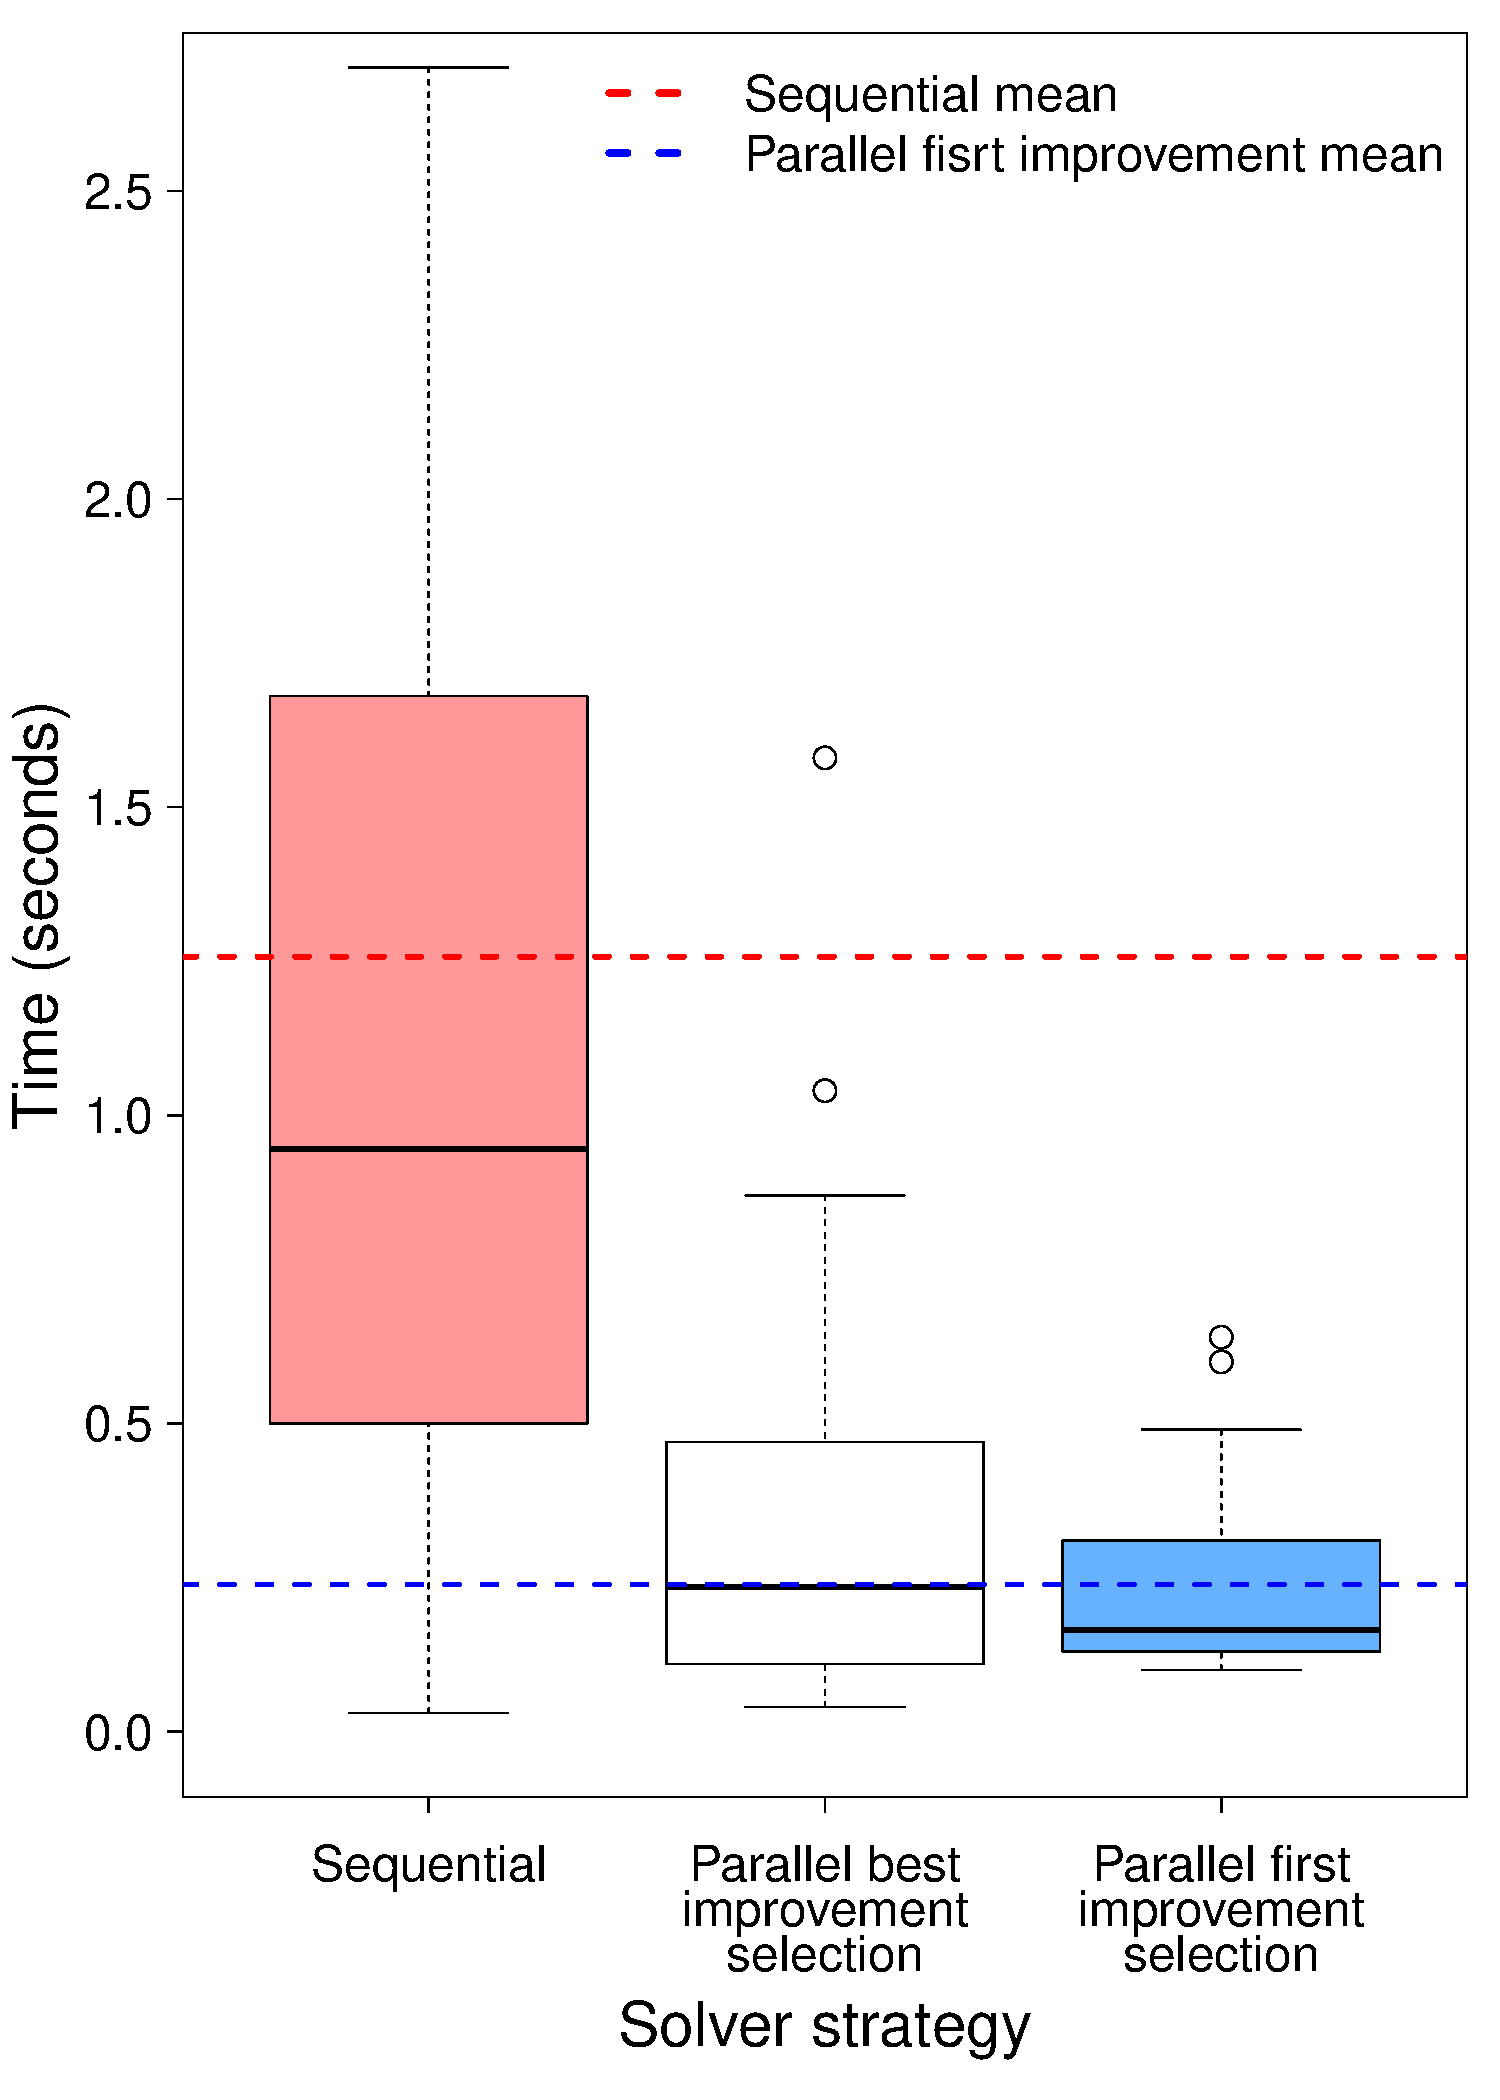
\includegraphics[width=0.8\textwidth]{g5_select_BP.pdf}
\caption{Comparison between sequential and parallel (best improvement and first improvement selections) runs to solve \SGP{} 5-3-7 using \posl}
\end{figure}

\begin{figure}[!h]
\centering
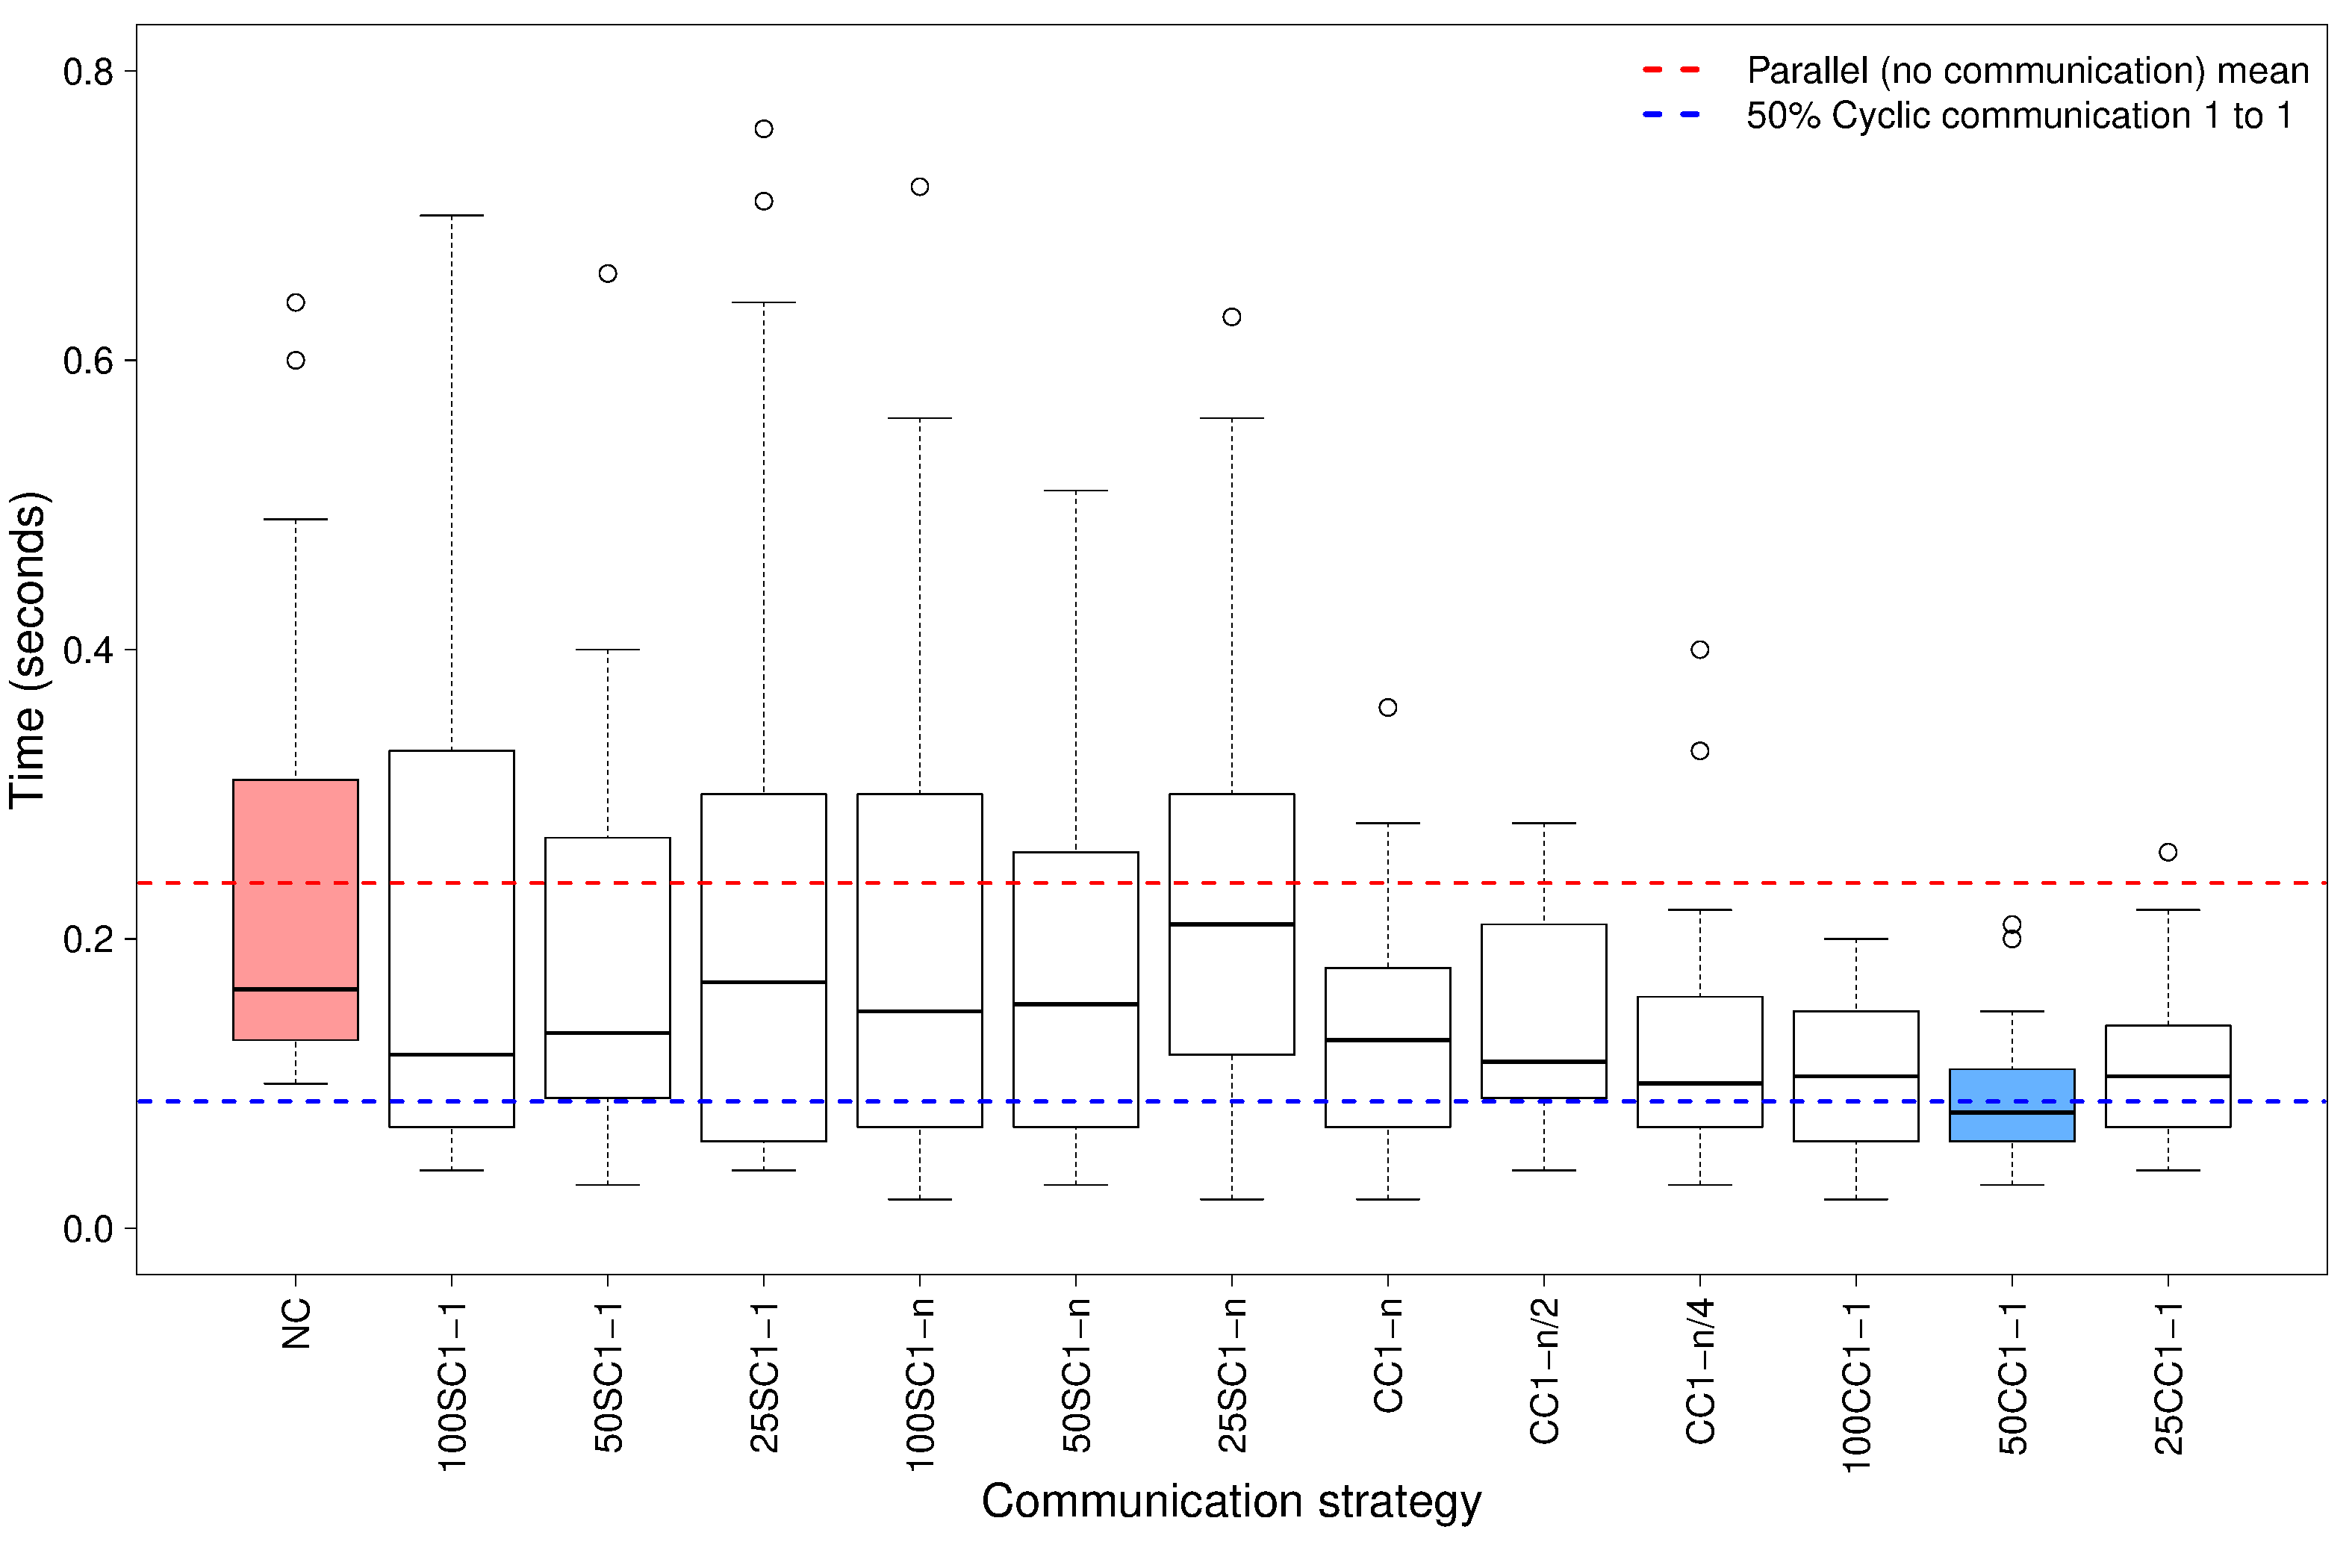
\includegraphics[width=0.8\textwidth]{g5_comm_BP.pdf}
\caption{Different communication strategies to solve \SGP{} 5-3-7 using \posl}\label{boxplot:5comm}
\end{figure}

\begin{figure}[!h]
\centering
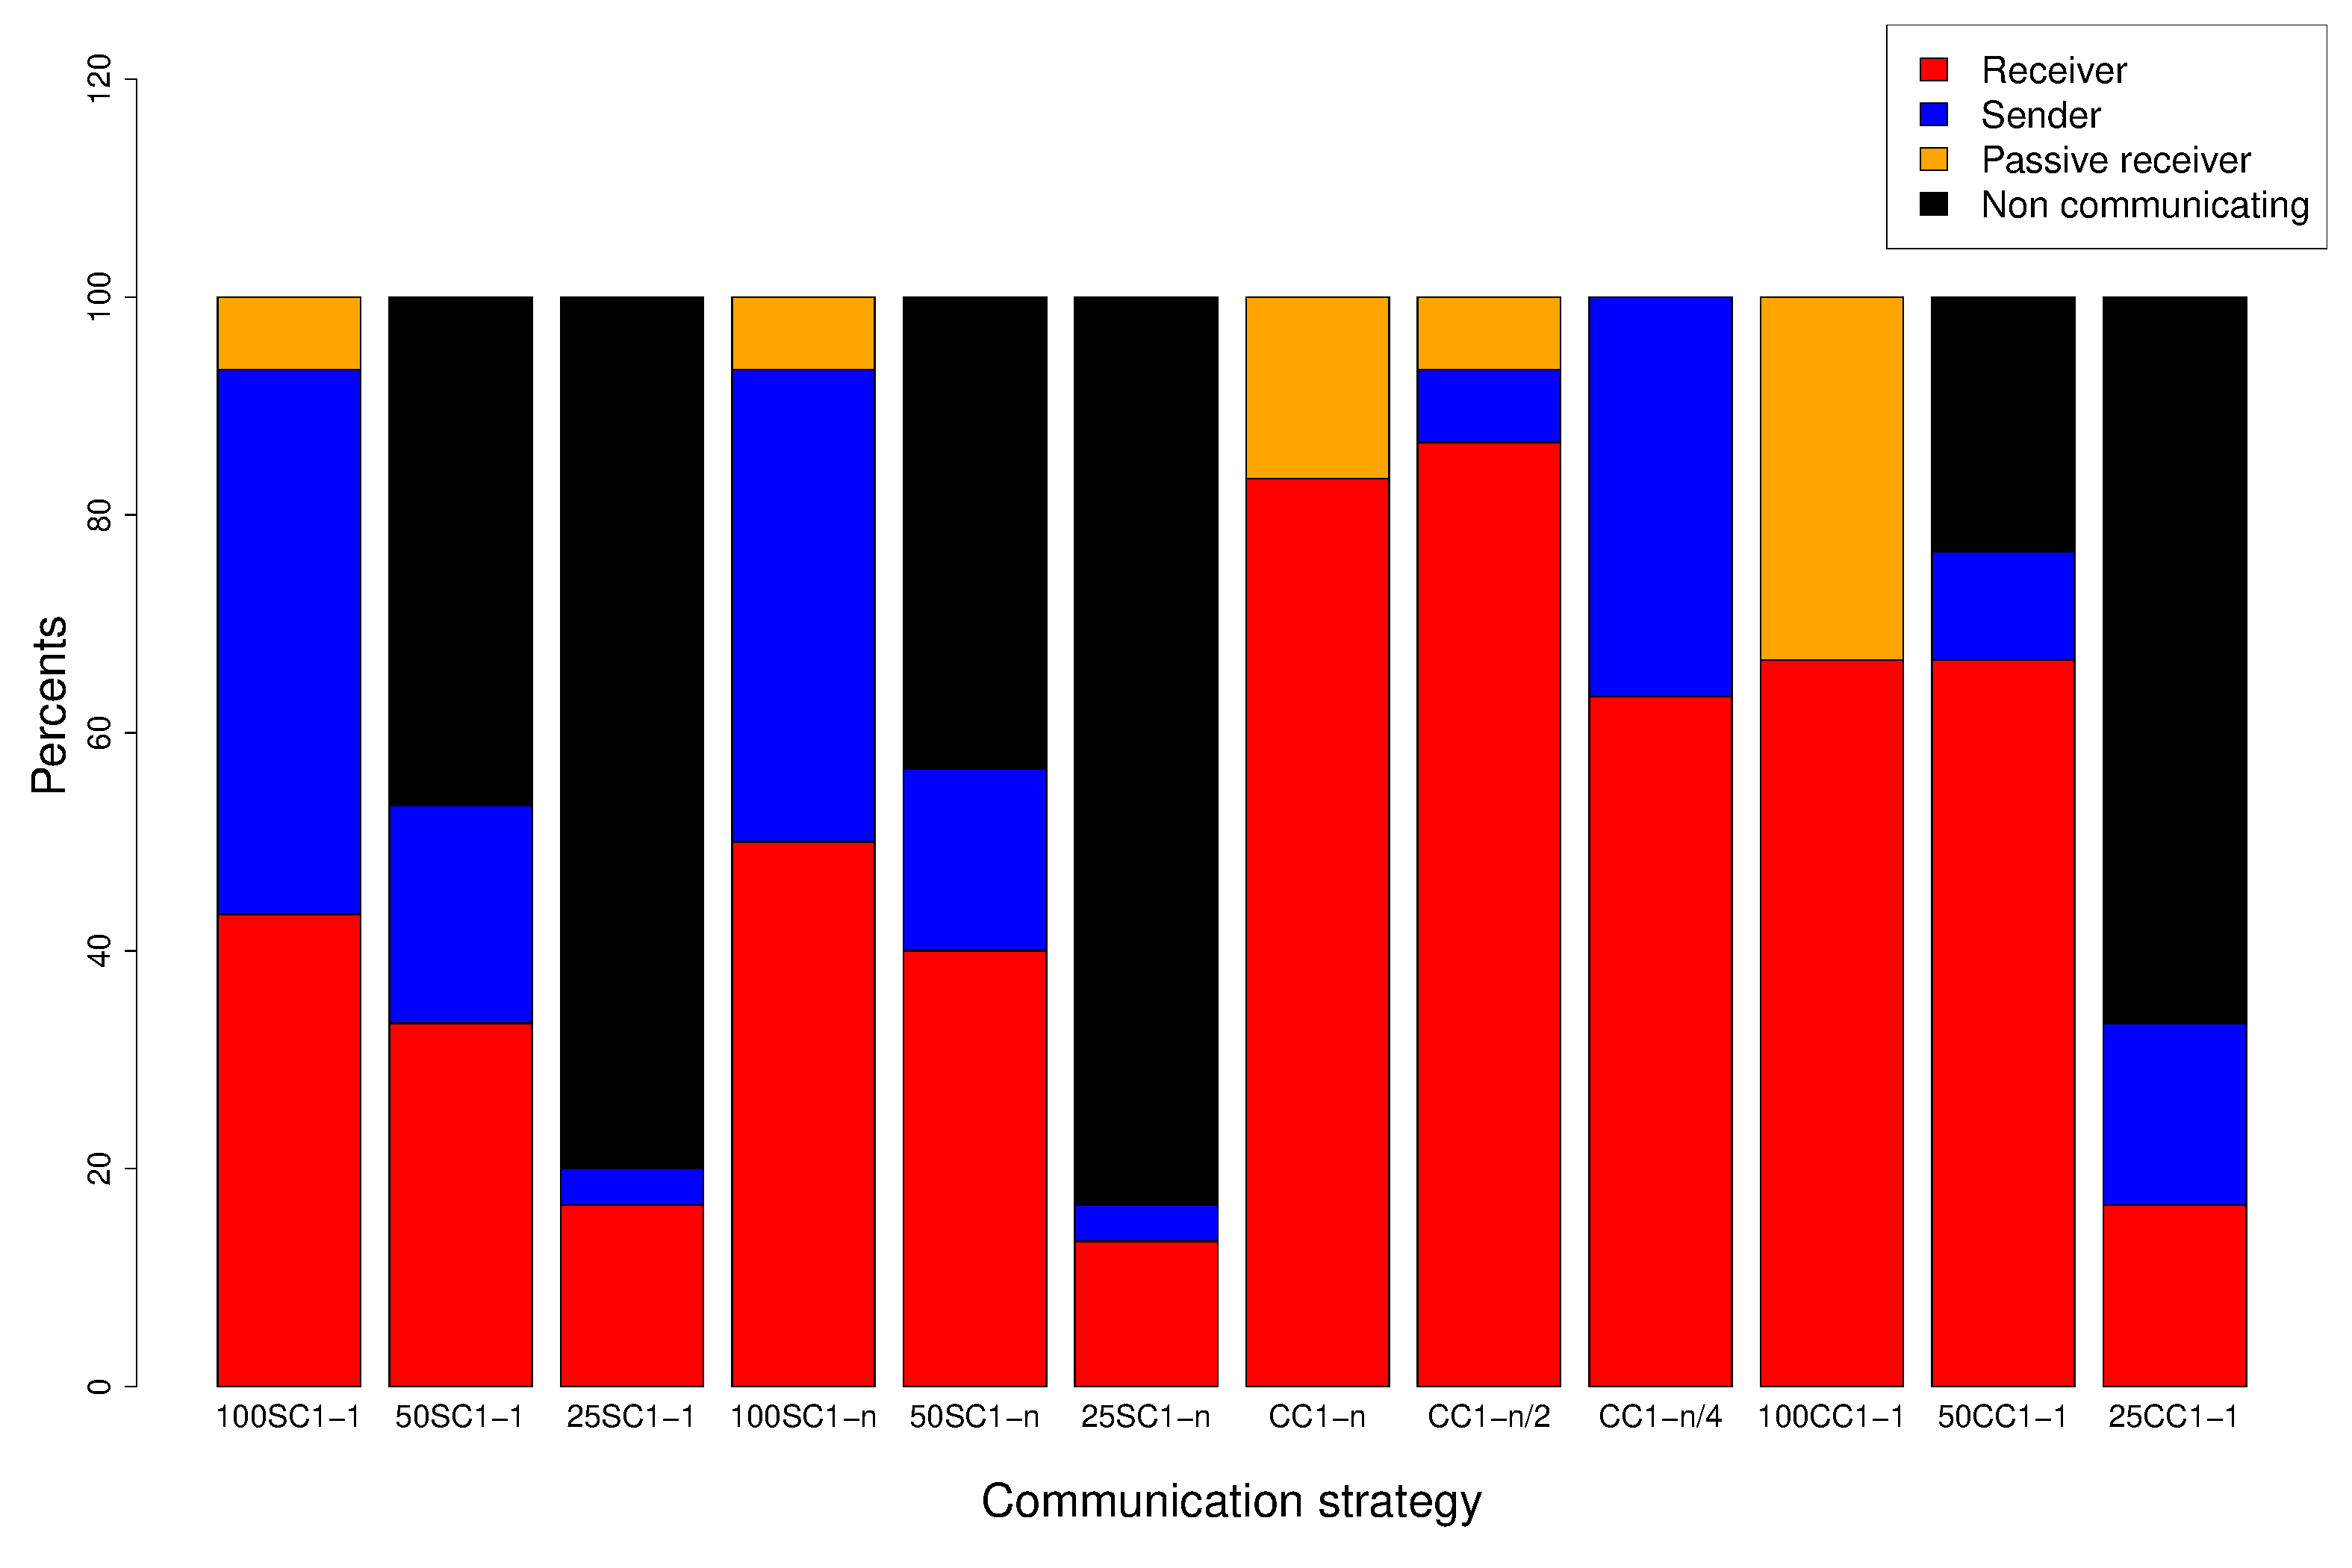
\includegraphics[width=0.8\textwidth]{g5_per_BP.pdf}
\caption{Solver proportion for each communication strategy to solve \SGP{} 5-3-7 using \posl}\label{barplot:5}
\end{figure}

%--------------------------------------

\begin{figure}[!h]
\centering
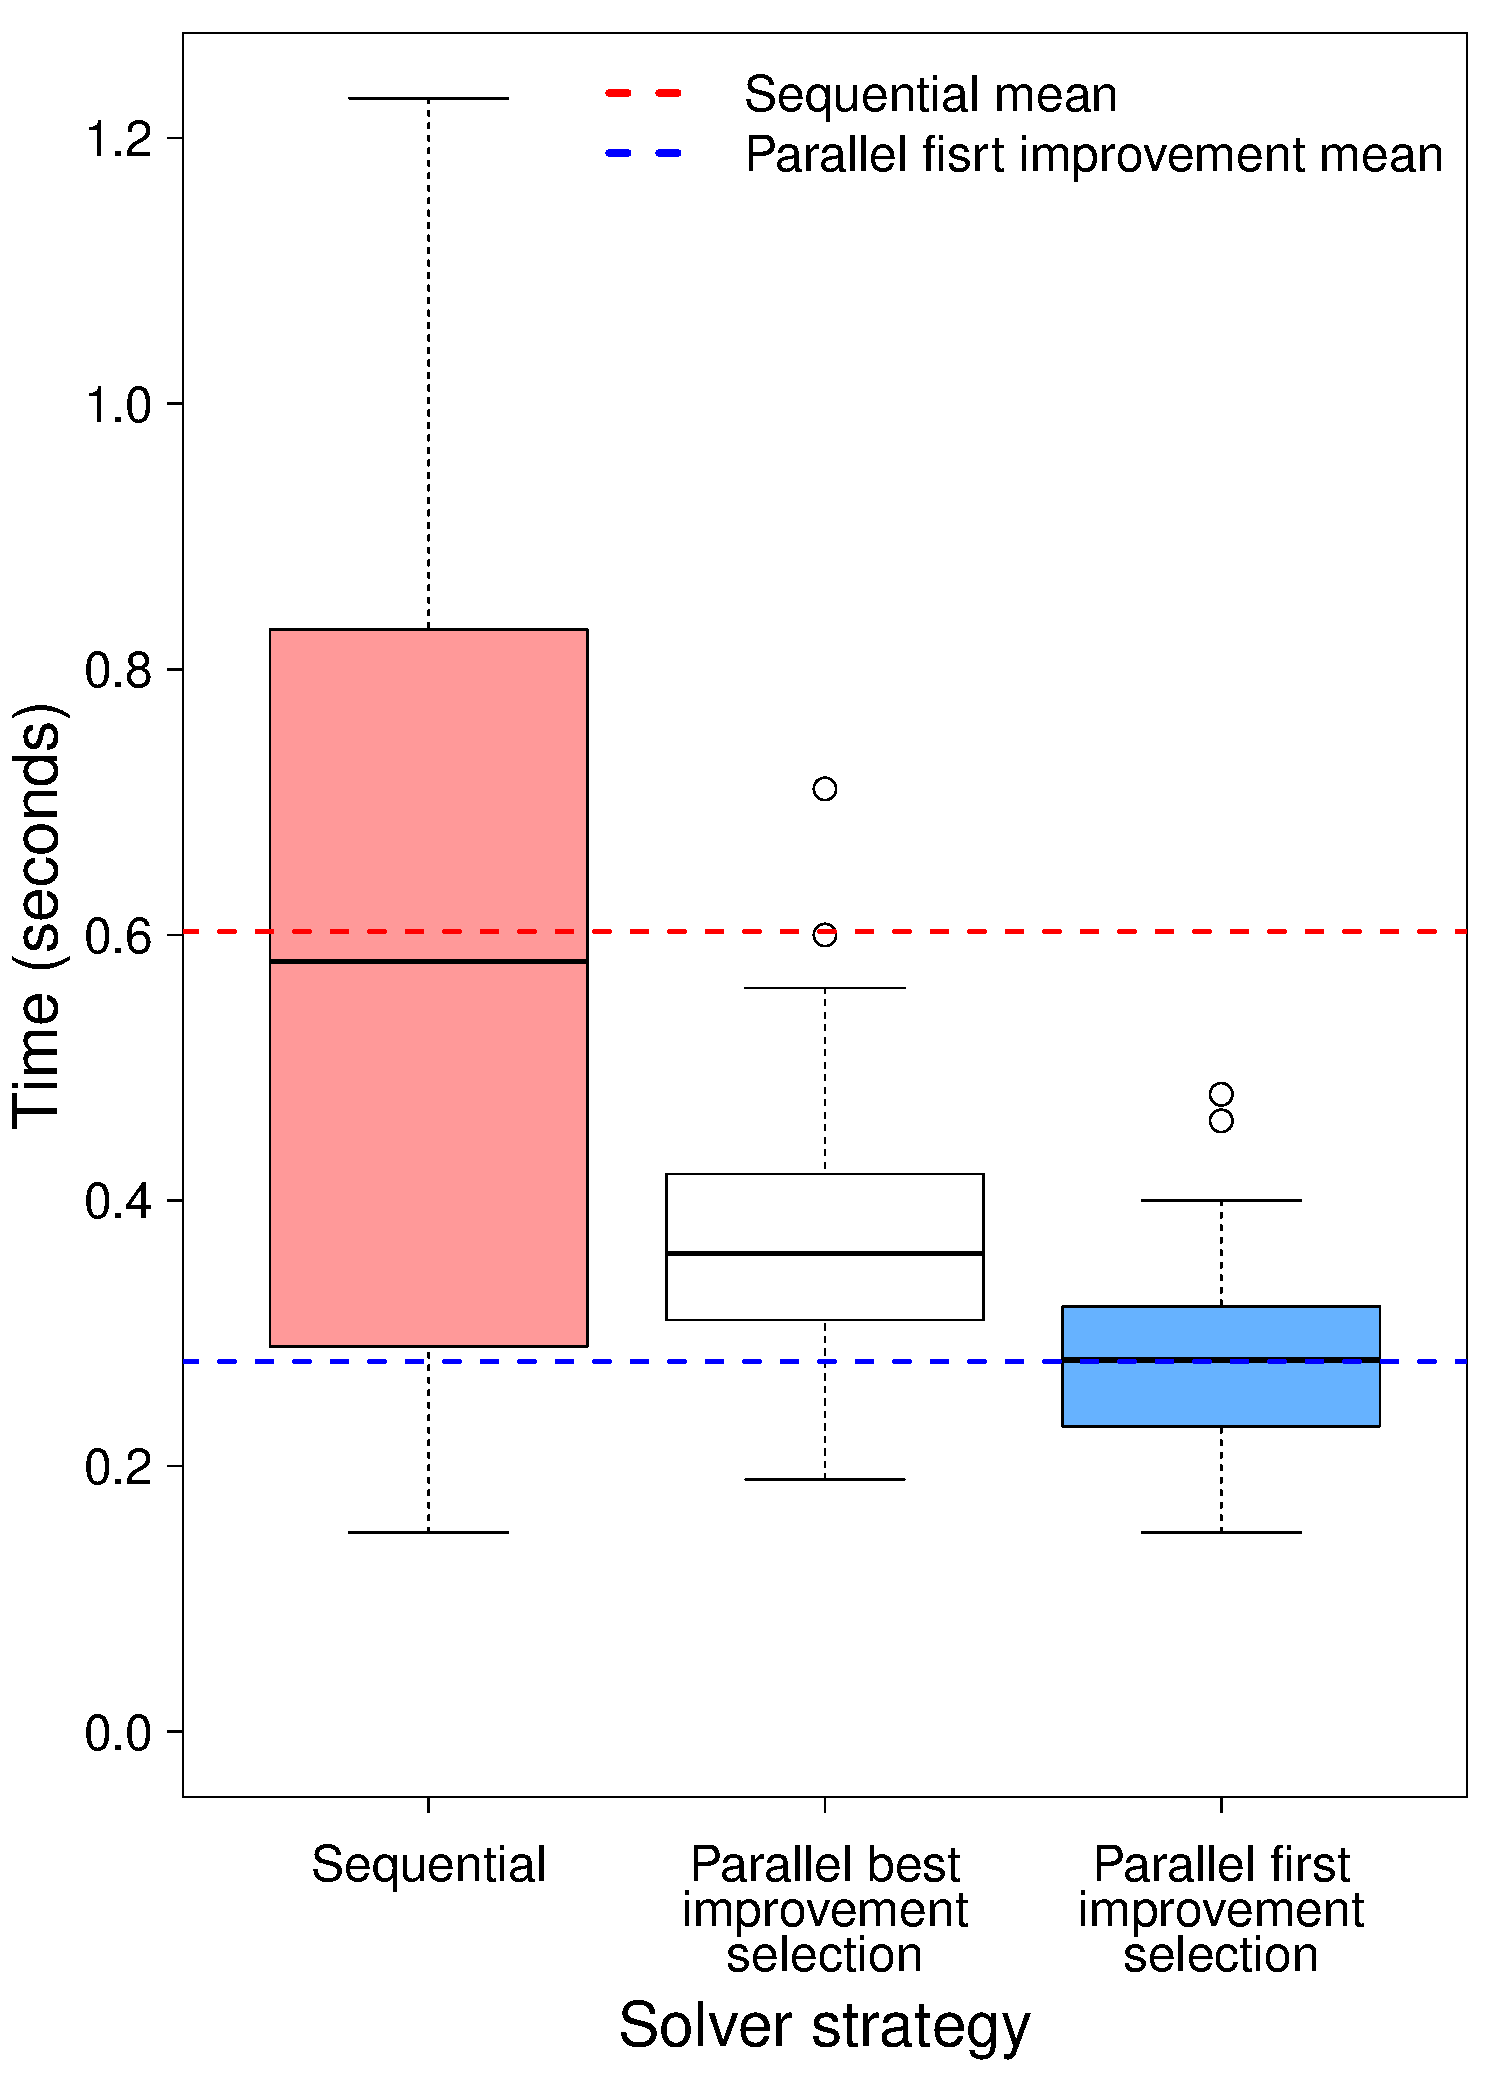
\includegraphics[width=0.75\textwidth]{g8_select_BP.pdf}
\caption{Comparison between sequential and parallel (best improvement and first improvement selections) runs to solve \SGP{} 8-4-7 using \posl}
\end{figure}

\begin{figure}[!h]
\centering
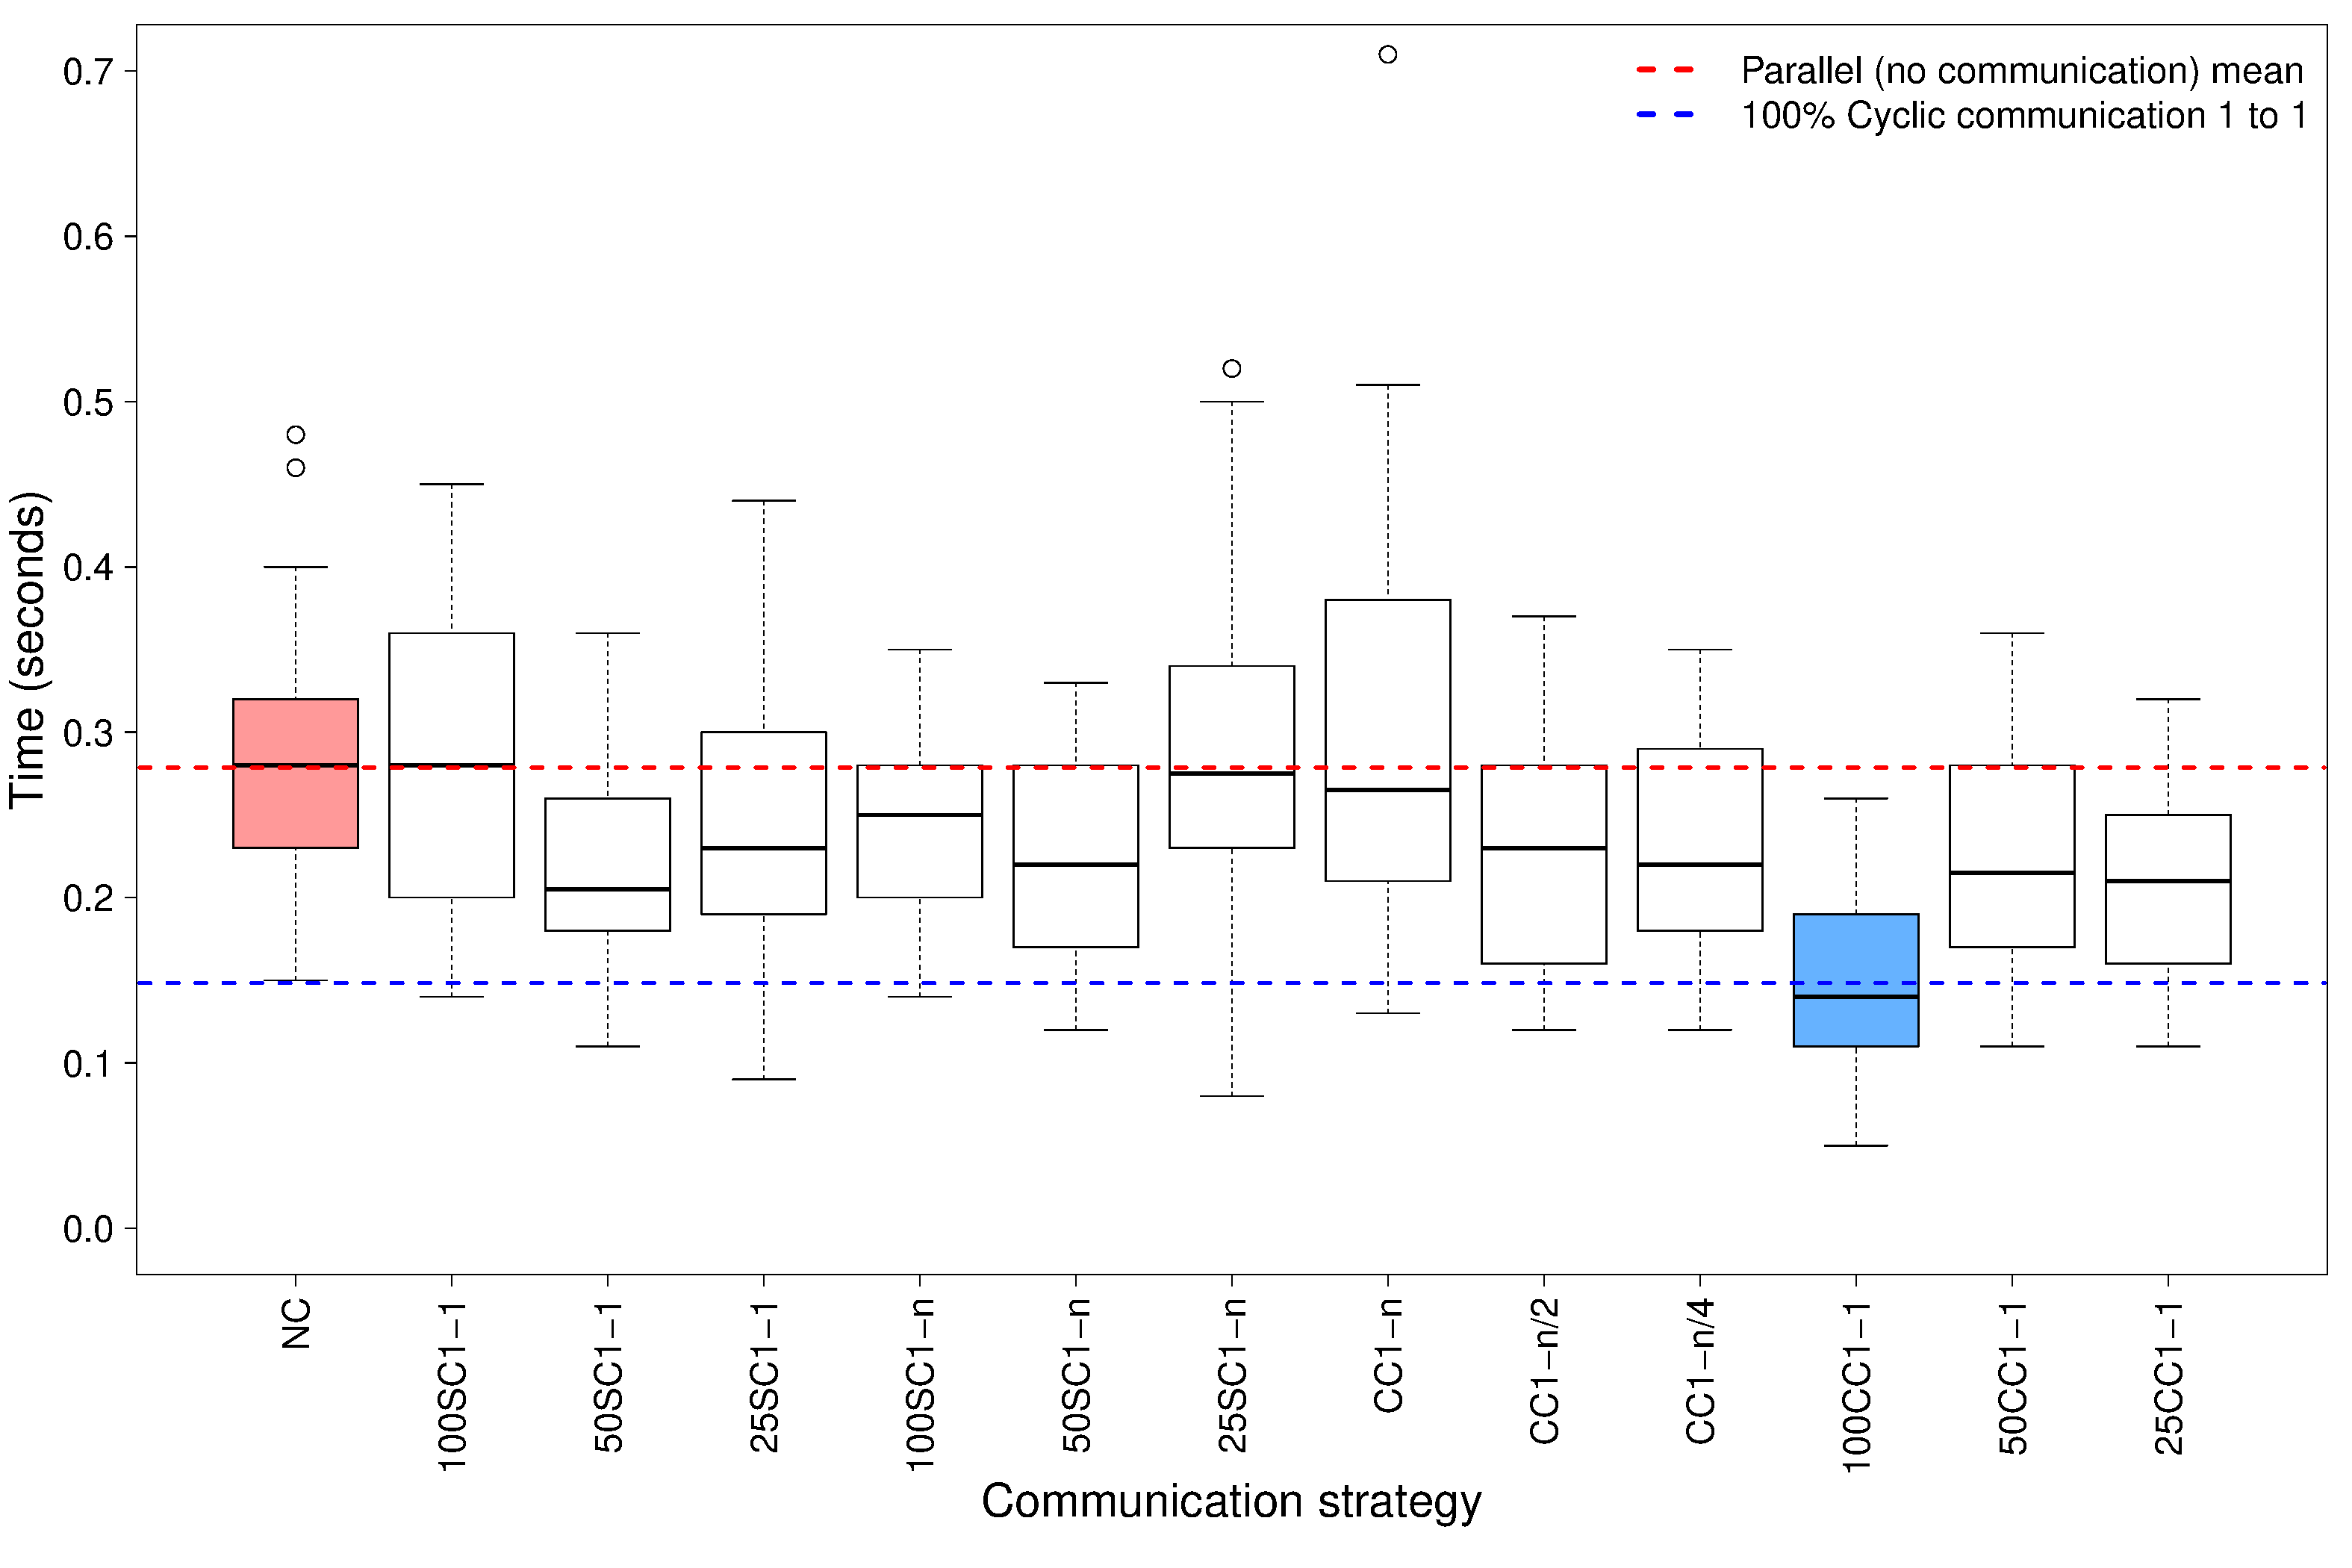
\includegraphics[width=0.75\textwidth]{g8_comm_BP.pdf}
\caption{Different communication strategies to solve \SGP{} 8-4-7 using \posl}\label{boxplot:8comm}
\end{figure}

\begin{figure}[!h]
\centering
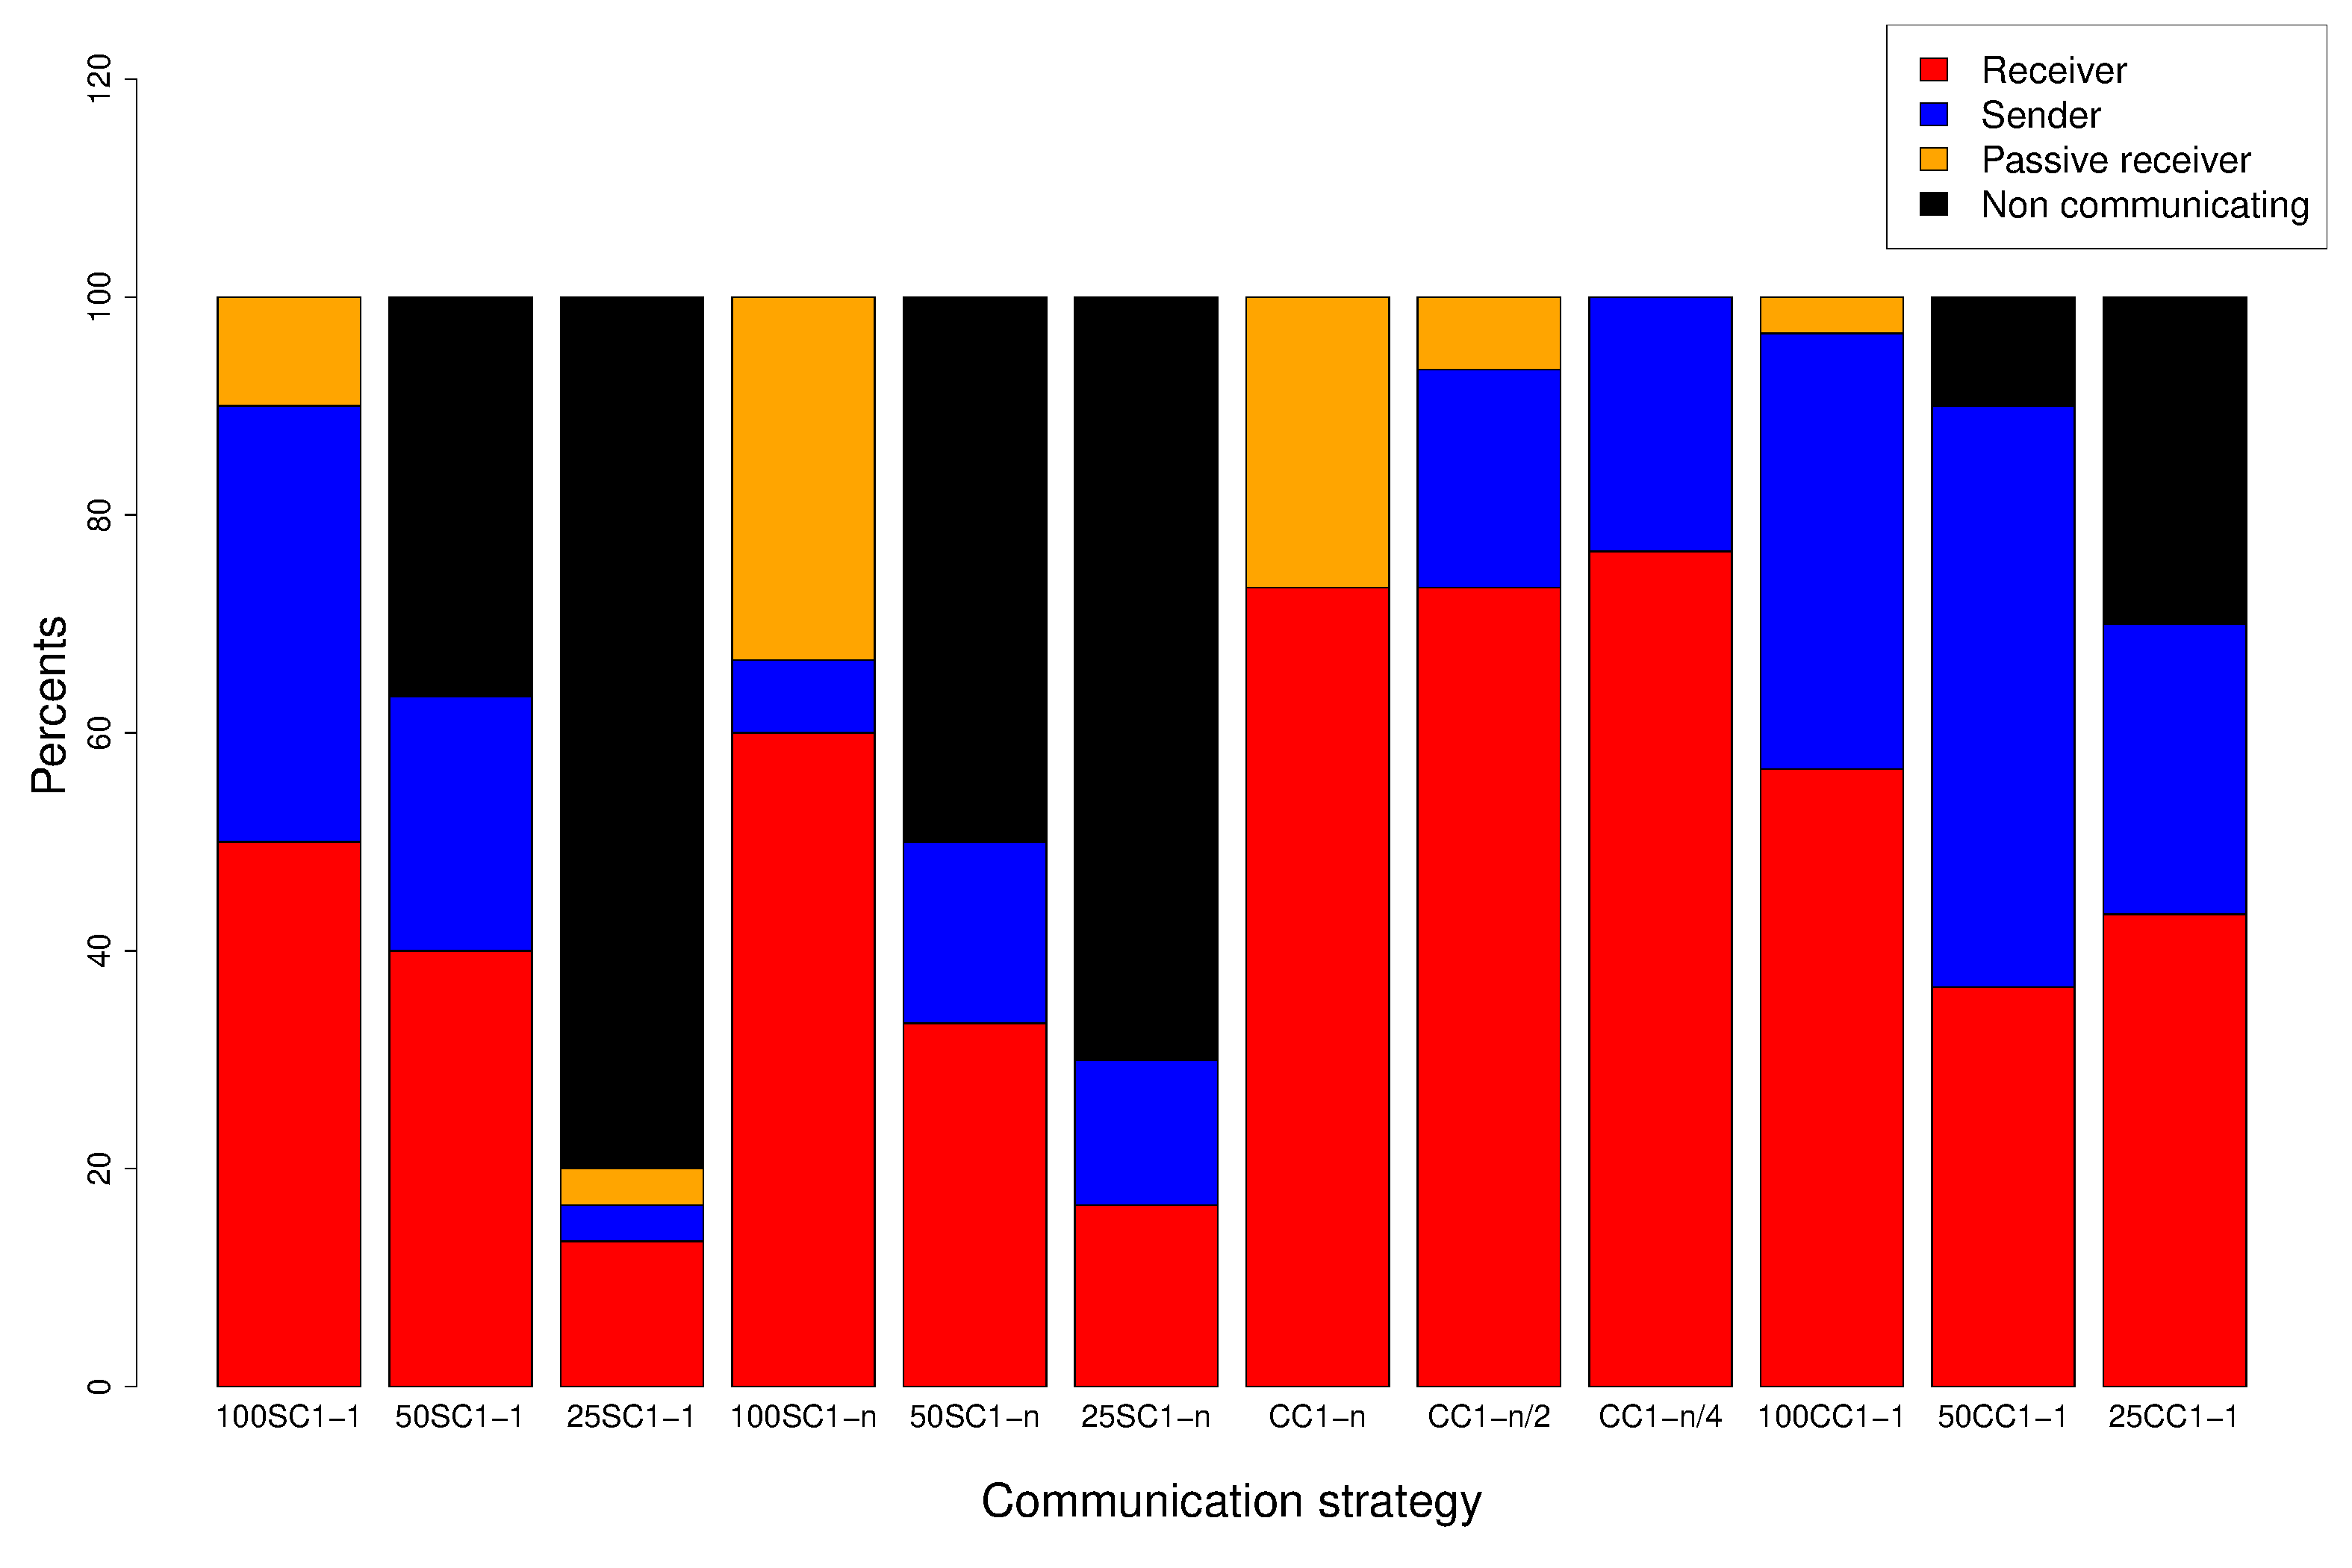
\includegraphics[width=0.8\textwidth]{g8_per_BP.pdf}
\caption{Solver proportion for each communication strategy to solve \SGP{} 8-4-7 using \posl}\label{barplot:8}
\end{figure}

%--------------------------------------

\begin{figure}[!h]
\centering
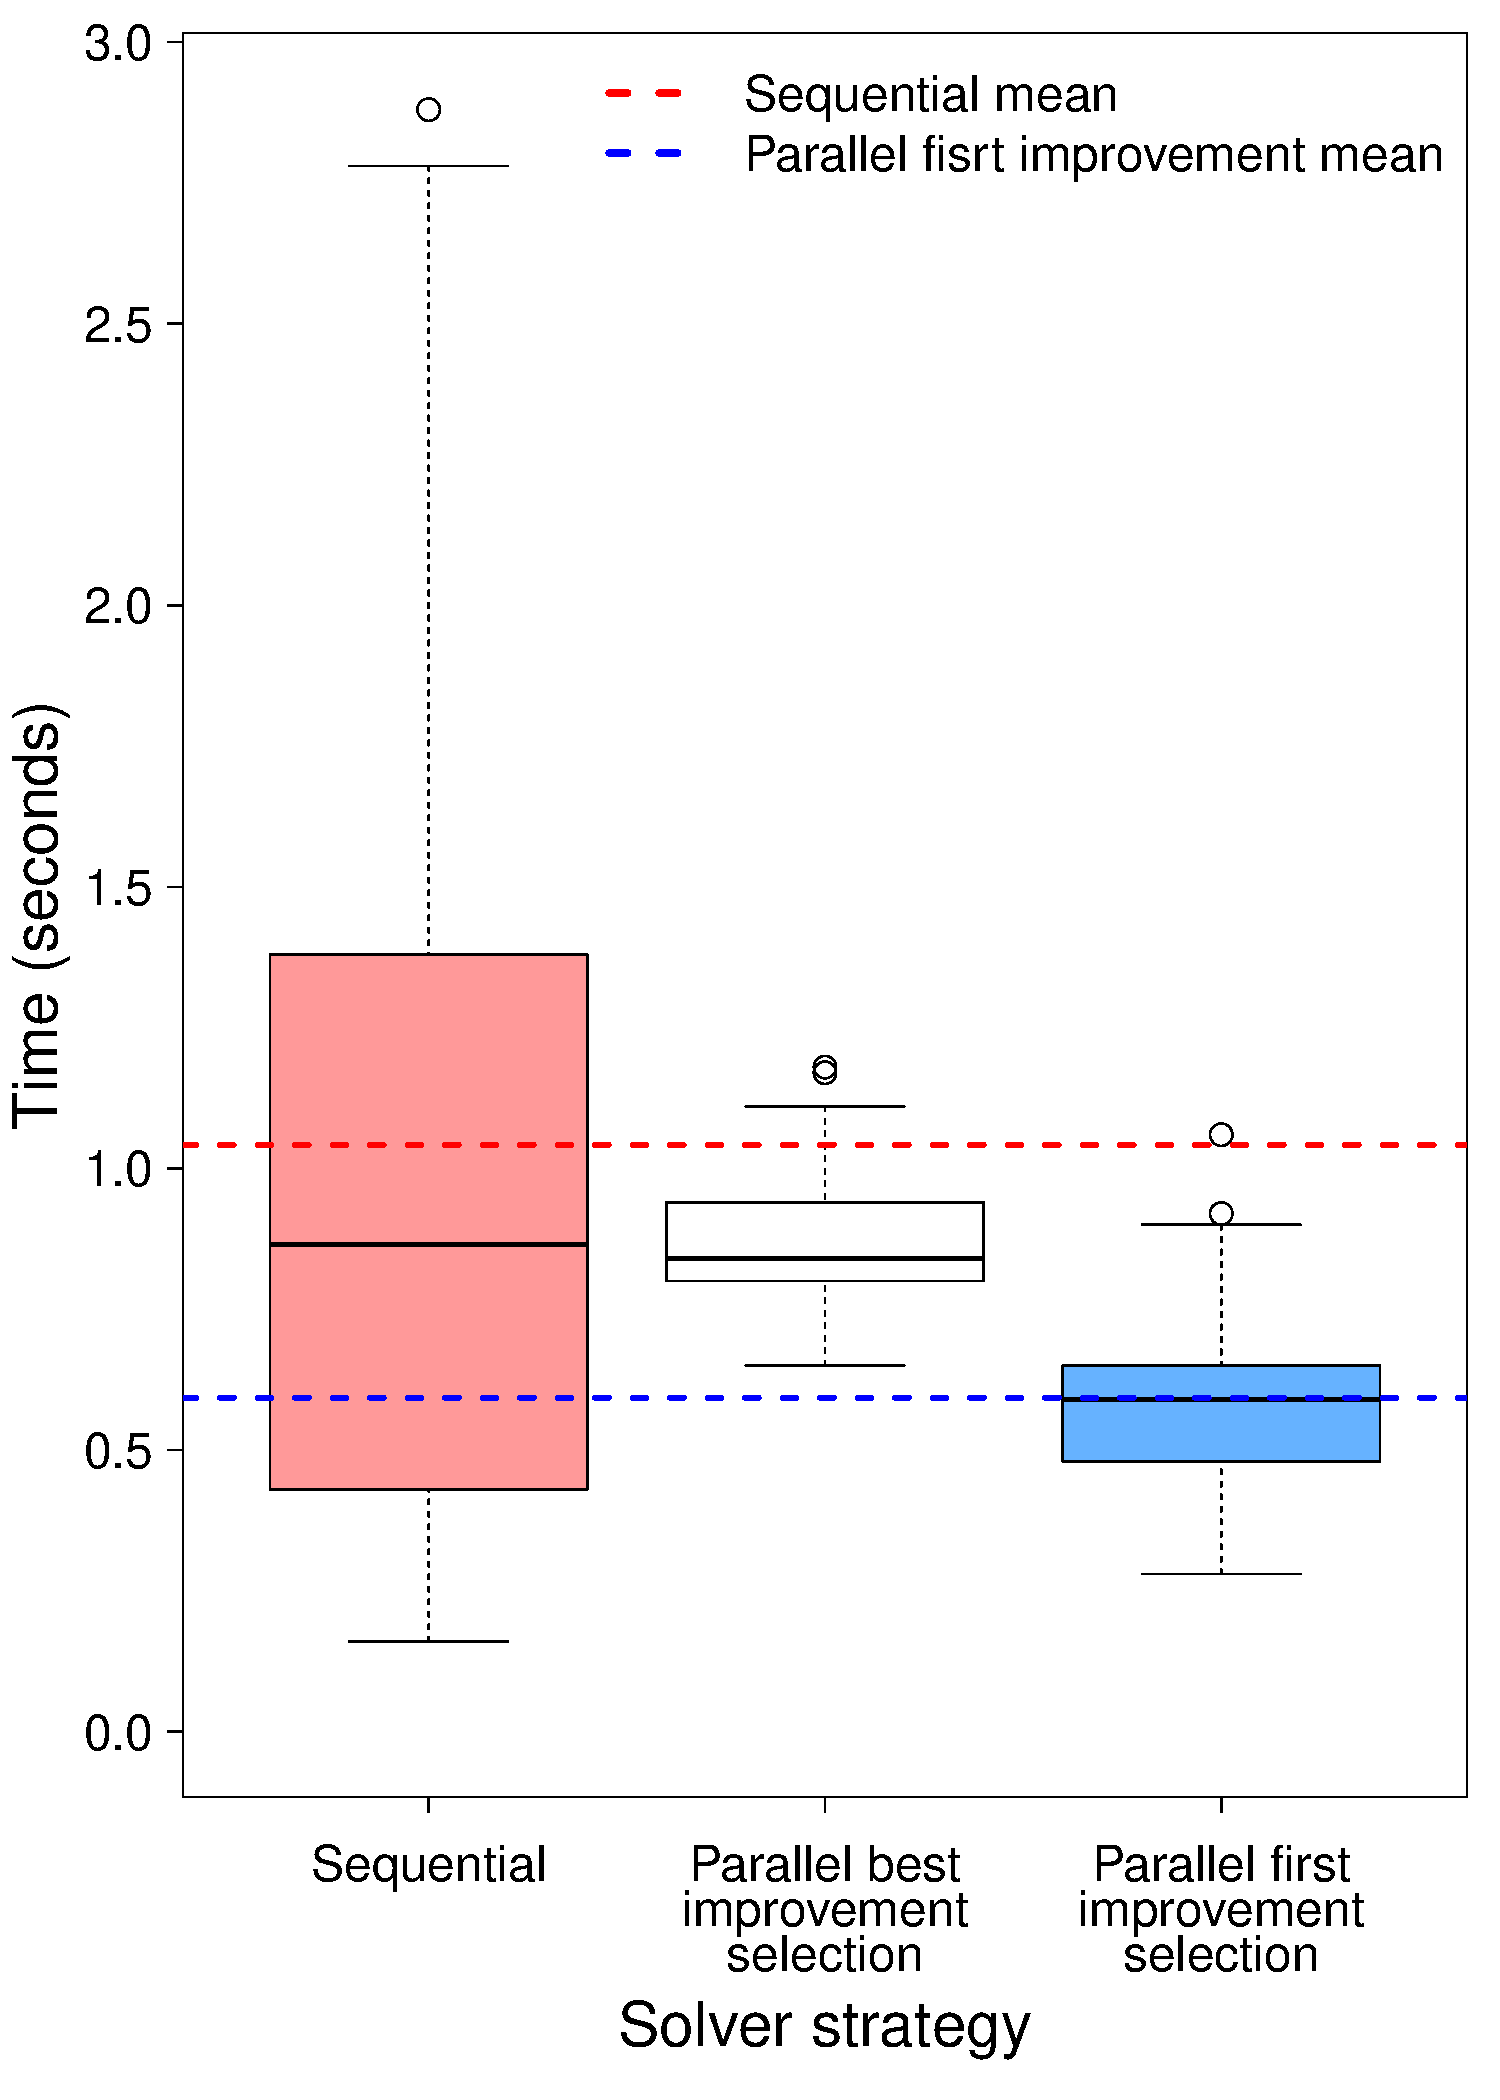
\includegraphics[width=0.75\textwidth]{g9_select_BP.pdf}
\caption{Comparison between sequential and parallel (best improvement and first improvement selections) runs to solve \SGP{} 9-4-8 using \posl}
\end{figure}

\begin{figure}[!h]
\centering
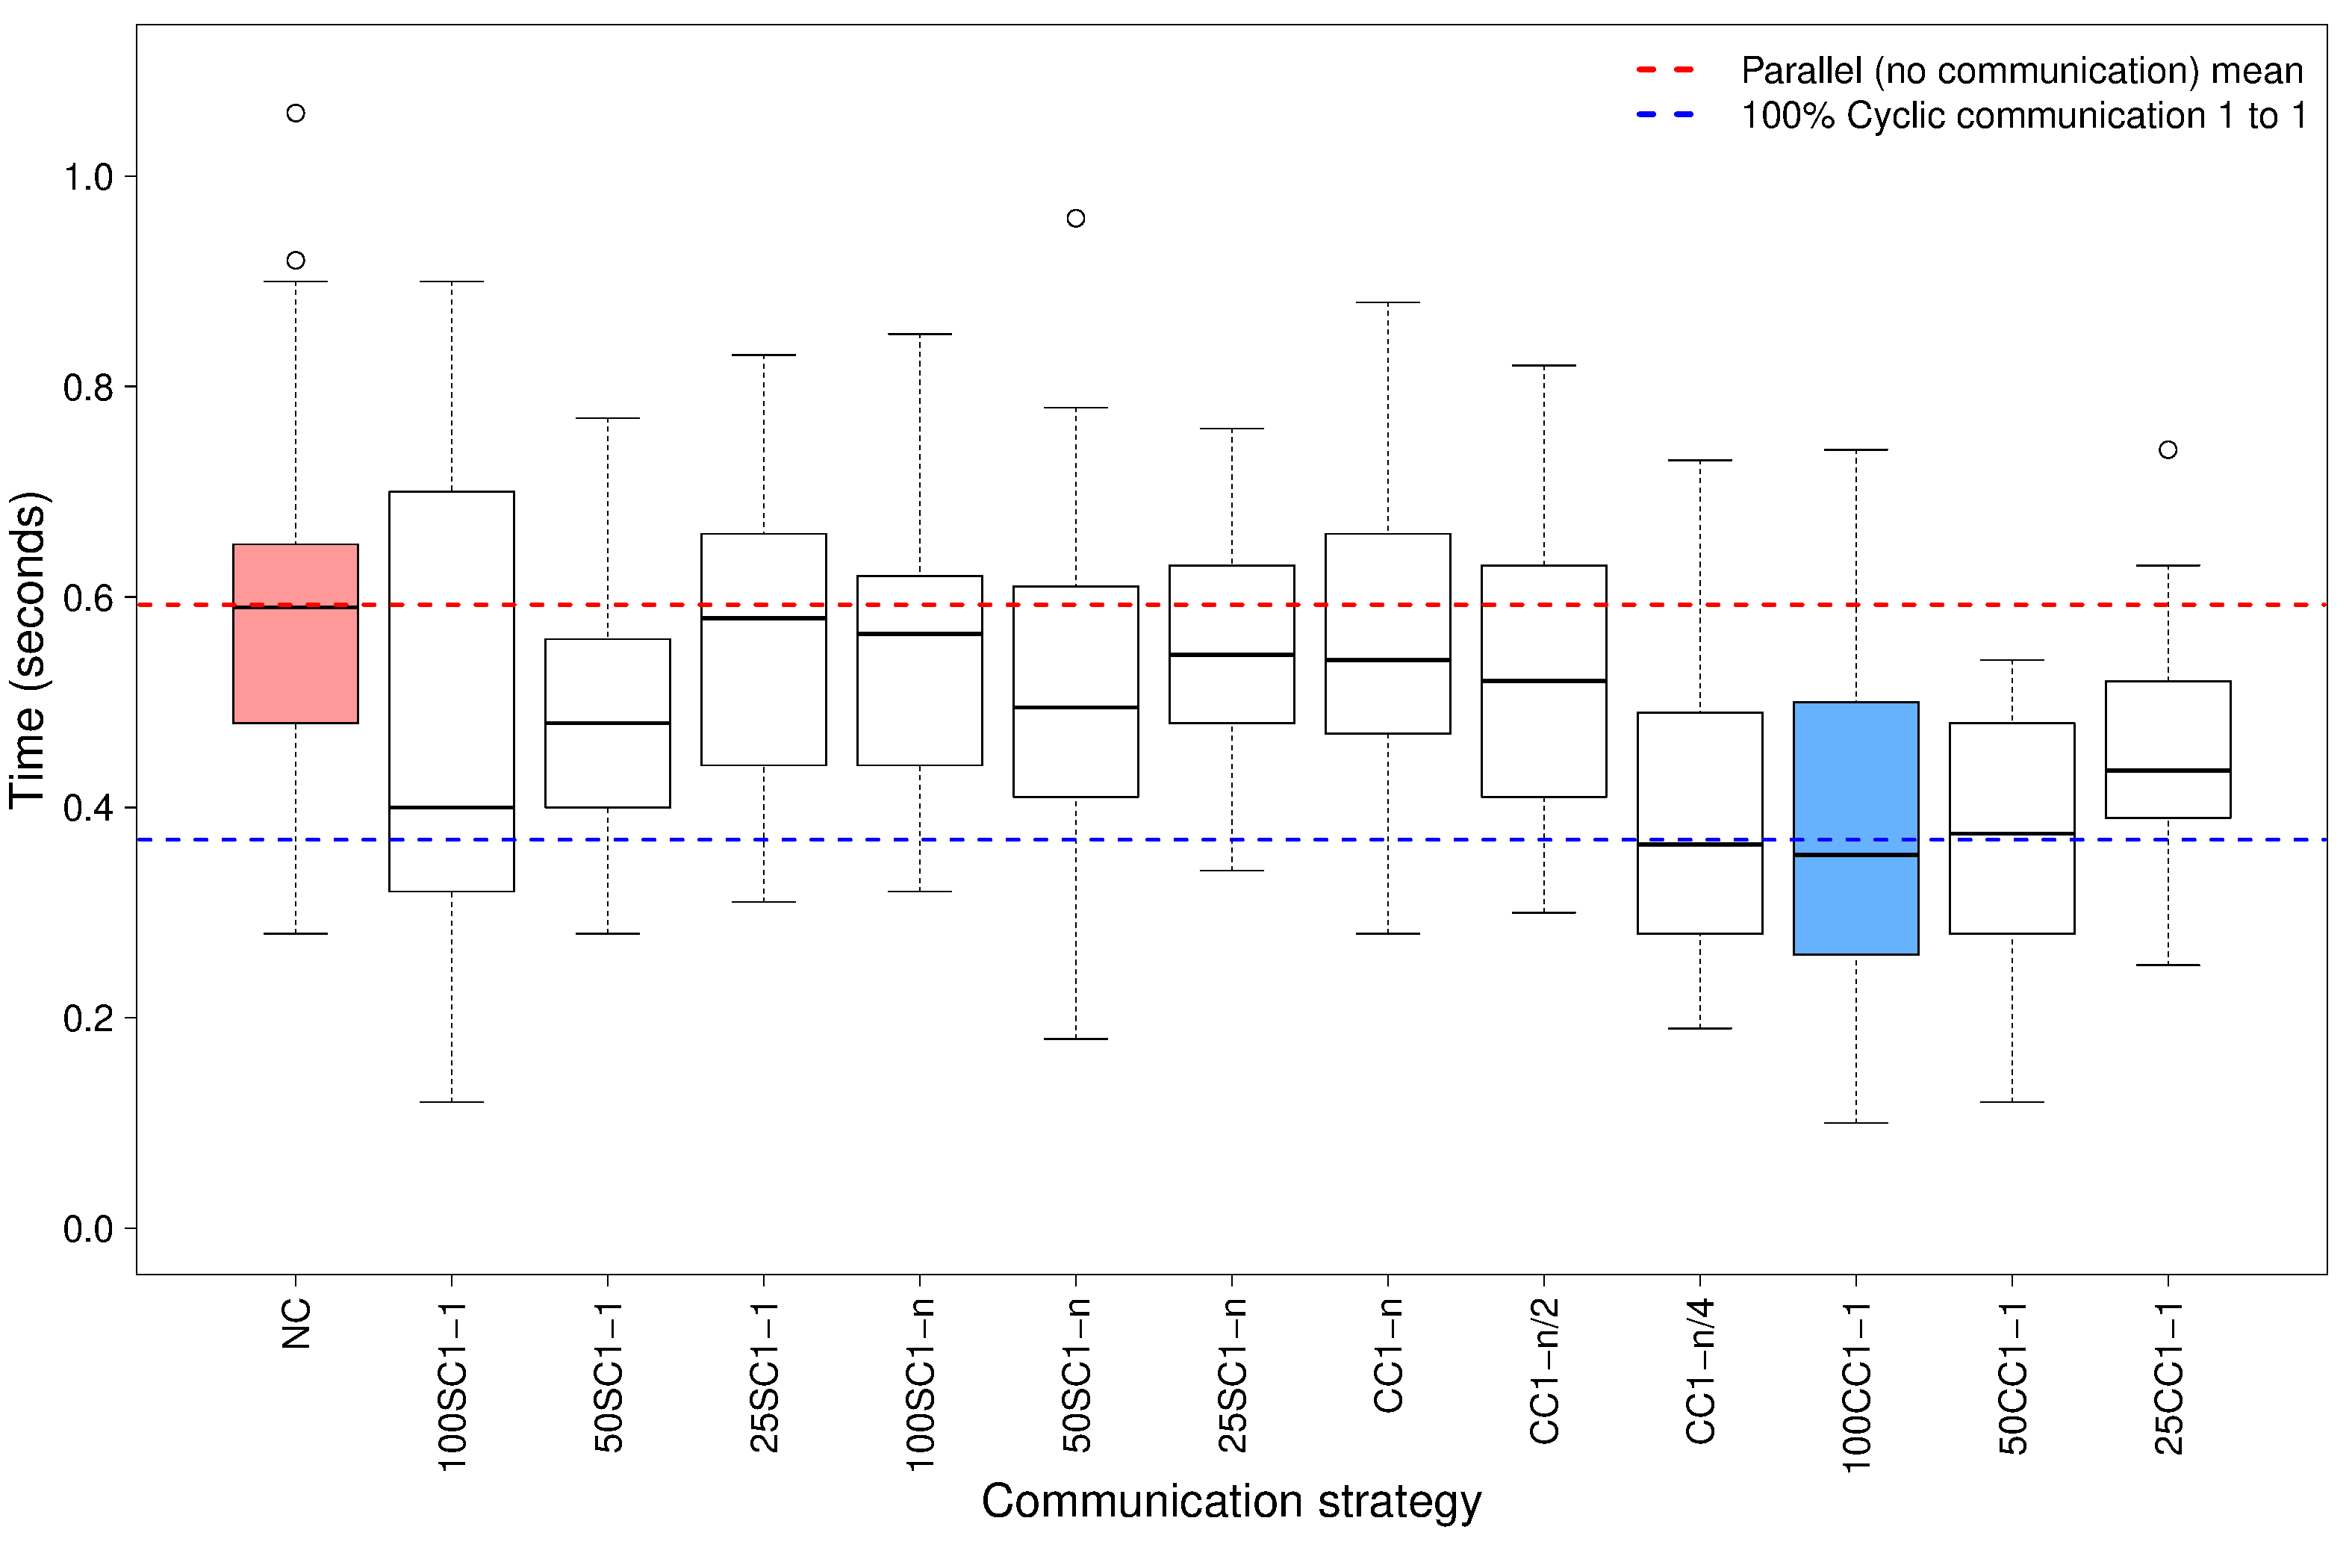
\includegraphics[width=0.75\textwidth]{g9_comm_BP.pdf}
\caption{Different communication strategies to solve \SGP{} 9-4-8 using \posl}\label{boxplot:9comm}
\end{figure}

\begin{figure}[!h]
\centering
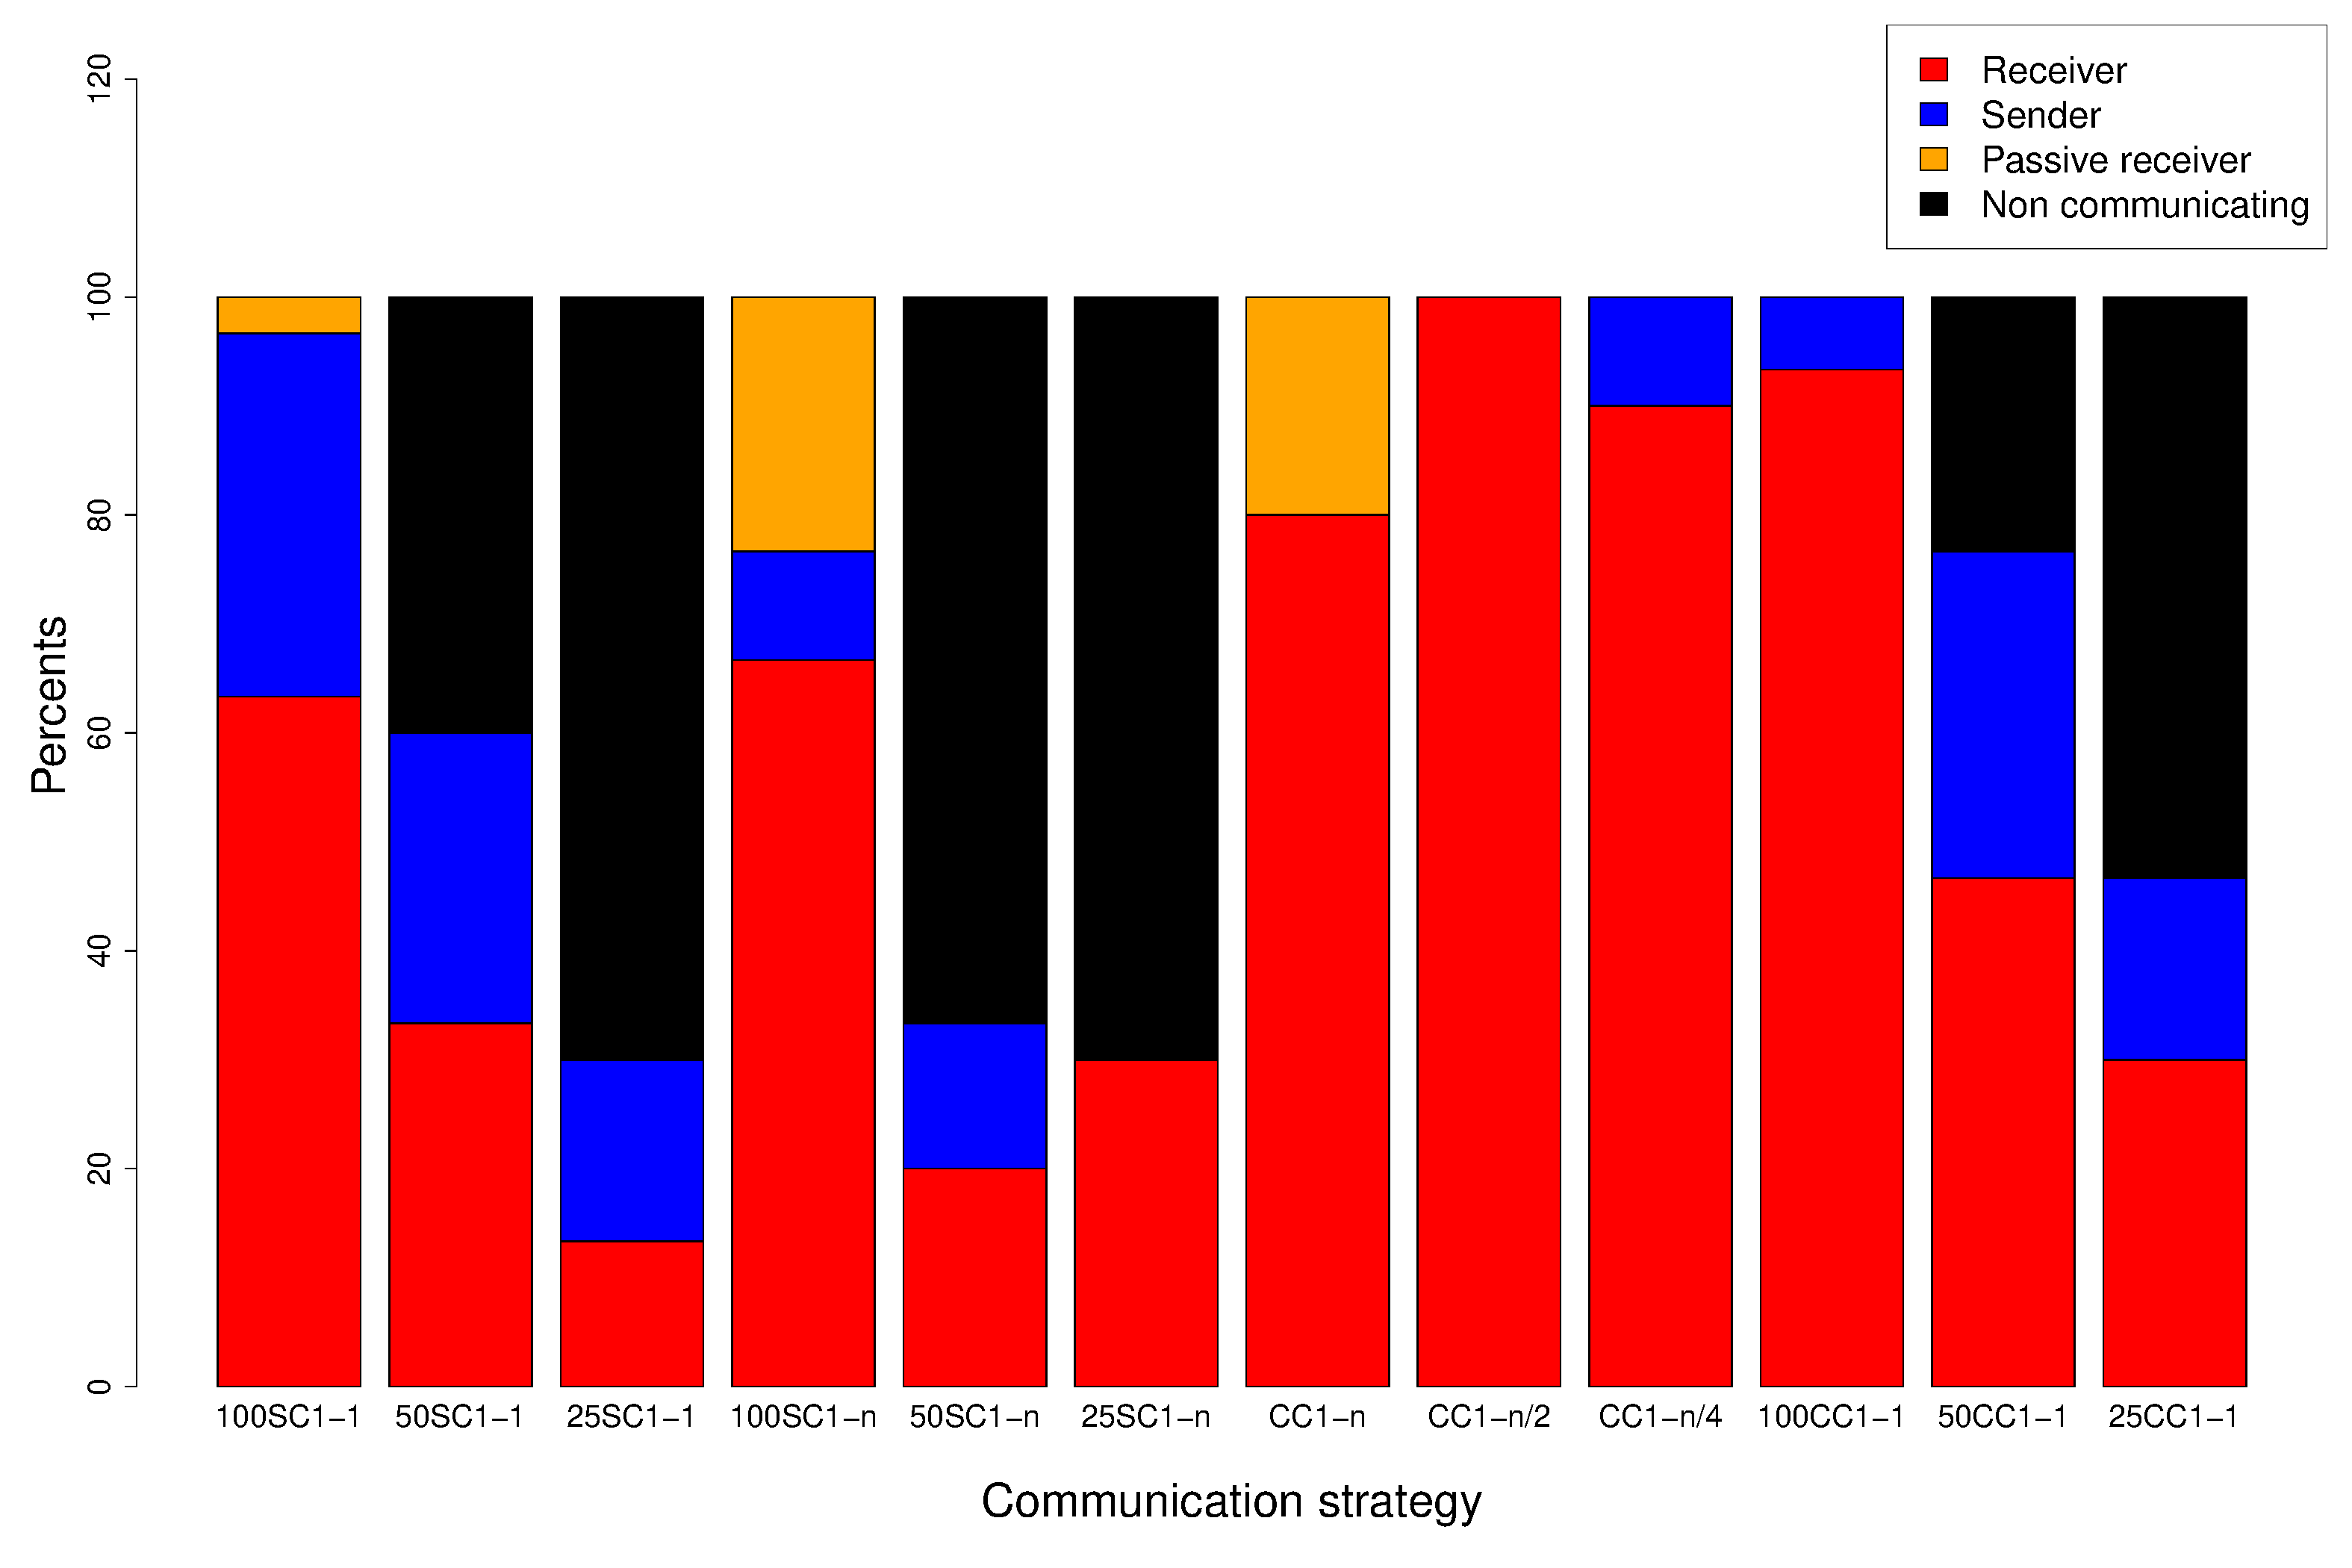
\includegraphics[width=0.8\textwidth]{g9_per_BP.pdf}
\caption{Solver proportion for each communication strategy to solve \SGP{} 9-4-8 using \posl}\label{barplot:9}
\end{figure}